% ============================================================
% Quantum Chemistry Chapter 2: The Particle in a Box
% 量子化学第二章：箱中粒子
% ============================================================

\documentclass[aspectratio=169,11pt]{beamer}

\usepackage{../../../theme/beamerthemeiqb}
\usepackage{../../../theme/iqb-layouts}
\renewcommand{\iqbheaderimage}{../../../theme/images/header.png}
\setstretch{1.05}

\usepackage{amsmath}
\usepackage{amssymb}
\usepackage[version=4]{mhchem}
\usepackage{booktabs}
\usepackage{array}
\usepackage{tikz}
\usetikzlibrary{shapes,arrows,positioning,calc,decorations.pathmorphing}

% Fix protein.png path for this subdirectory
\renewcommand{\iqbsectionframe}[2]{%
  \setsection{#1}%
  \begin{frame}[plain,noframenumbering]
    \begingroup
      % Hide footer on section divider
      \setbeamertemplate{footline}{}
      % Background gradient
      \begin{tikzpicture}[remember picture,overlay]
        \fill[white] (current page.south west) rectangle (current page.north east);
        \shade[left color=white, right color=iqblightgray!30]
              (current page.south west) rectangle (current page.north east);
      \end{tikzpicture}
      % Left vertical bar
      \begin{tikzpicture}[remember picture,overlay]
        \draw[line width=8pt, color=iqbblue]
             (current page.north west) -- (current page.south west);
      \end{tikzpicture}
      % Decorative protein (FIXED PATH)
      \begin{tikzpicture}[remember picture,overlay]
        \node[anchor=south east, inner sep=0pt, opacity=0.12]
             at ($(current page.south east) + (-1cm, 1cm)$) {
          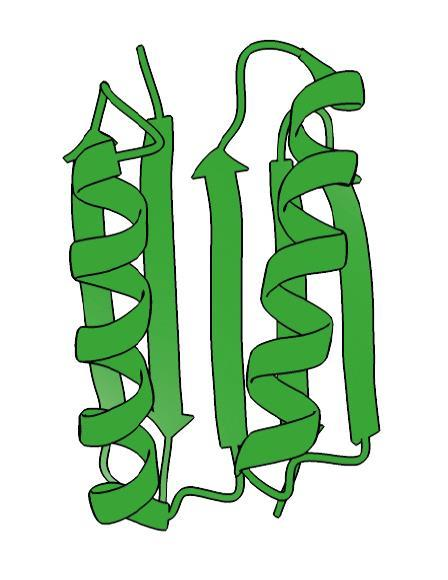
\includegraphics[height=5cm,keepaspectratio]{../../../theme/images/protein.png}
        };
      \end{tikzpicture}
      % Title
      \vspace*{0.5cm}
      \begin{center}
        {\Huge\color{iqbblue}\textbf{#2}}\\[0.3cm]
        {\Large\color{iqbgray}#1}
      \end{center}
      \vspace*{0.3cm}
    \endgroup
  \end{frame}
}

% 缩小子项缩进（本课程讲义使用更紧凑的层级）
\renewcommand{\subitem}[1]{%
  \par\vspace{2pt}%
  \noindent\hspace{0.8em}\textcolor{iqbblue}{$\circ$}\ #1%
}


% 设置教材信息
\iqbtextbook{Quantum Chemistry}{Levine}{7th Edition}{Pearson}

% 课程讲义元数据
\lecturetitle{第二章：箱中粒子}
\lectureengtitle{Chapter 2: The Particle in a Box}

\author{东山月光下QM小组}
\date{\today}

\begin{document}

% ============================================================
% Footer Configuration
% ============================================================
\iqbfootline{default}{title}{pageofy}

% ------------------------------------------------------------
% 1. Cover
% ------------------------------------------------------------
\iqbcoverframe

% ------------------------------------------------------------
% 目录
% ------------------------------------------------------------
\begin{frame}{本章内容}
  \iqblayouttwo{
    \iqbsectiontitle{一维箱中粒子}
    \begin{iqbitemize}
      \item \textbf{2.1 引言：模型的重要性}（Introduction）
      \item \textbf{2.2 问题设定}（Problem Setup）
      \item \textbf{2.3 薛定谔方程求解}（Solving the Schrödinger Equation）
      \item \textbf{2.4 边界条件}（Boundary Conditions）
      \item \textbf{2.5 波函数与能级}（Wave Functions and Energy Levels）
    \end{iqbitemize}
  }{
    \iqbsectiontitle{深入分析}
    \begin{iqbitemize}
      \item \textbf{2.6 概率密度}（Probability Density）
      \item \textbf{2.7 期望值}（Expectation Values）
      \item \textbf{2.8 不确定性验证}（Uncertainty Verification）
      \item \textbf{2.9 三维箱中粒子}（Three-Dimensional Box）
      \item \textbf{2.10 简并性}（Degeneracy）
    \end{iqbitemize}
  }
\end{frame}

% ============================================================
% Part 1: Introduction (2.1)
% ============================================================
\iqbsectionframe{Introduction}{箱中粒子模型引言}

% ------------------------------------------------------------
% 2.1-1. Why Study This Model?
% ------------------------------------------------------------
\begin{frame}{为什么研究箱中粒子？}
  \iqbfontsizemode{small}

  \iqblayouttwo{
    \iqbsectiontitle{最简单的量子系统}
    \begin{iqbitemize}
      \item 箱中粒子是量子力学的\textbf{最简单}非平凡模型
      \item 数学形式简单，可以精确求解并得到\textbf{解析解}（analytical solution）
      \item 展现量子力学的基本特征：\textbf{能量量子化}（energy quantization）、\textbf{零点能}（zero-point energy）、概率分布
      \item 是理解更复杂量子系统的重要起点和基础
    \end{iqbitemize}

    \iqbsep

    \iqbsectiontitle{教学价值}
    \begin{iqbitemize}
      \item 帮助理解量子化概念如何从边界条件自然产生
      \item 直观展示波函数的物理意义和概率诠释
      \item 演示期望值和不确定性的计算方法
      \item 为氢原子、谐振子等复杂系统奠定基础
    \end{iqbitemize}
    
    \iqbtinysep

    \iqbgreenbox{关键意义}{箱中粒子是理解量子力学的\textbf{入门钥匙}}
  }{
    \iqbsectiontitle{实际应用：共轭分子}
    \begin{iqbitemize}
      \item \textbf{共轭多烯}（conjugated polyenes）的$\pi$电子体系可用一维箱中粒子模型近似处理
      \item 丁二烯包含4个碳原子的共轭体系，\textbf{吸收光谱}（absorption spectrum）可用模型预测
      \item $\beta$-胡萝卜素是长链共轭分子，吸收可见光呈现橙色
      \item 视紫红质是视网膜中的共轭分子，在视觉过程中起关键作用
      \item 箱中模型能够定性地预测吸收光谱并与实验结果吻合
    \end{iqbitemize}

    \iqbtinysep

    \iqbsectiontitle{其他应用领域}
    \begin{iqbitemize}
      \item \textbf{量子点}：纳米尺度的半导体晶体，其尺寸决定发光颜色
      \item \textbf{纳米材料}：石墨烯量子点、碳纳米管等低维材料研究
      \item \textbf{核物理}：核子在有限核势阱中运动的简化模型
      \item \textbf{超晶格}：人工制备的周期性结构，用于量子阱器件
    \end{iqbitemize}
  }
\end{frame}

% ============================================================
% Part 2: The Problem (2.2)
% ============================================================
\iqbsectionframe{The Problem}{问题设定}

% ------------------------------------------------------------
% 2.2-1. Potential Energy Function
% ------------------------------------------------------------
\begin{frame}{势能函数：定义问题}
  \iqblayouttwo{
    \iqbsectiontitle{一维无限深势阱}
    \begin{iqbitemize}
      \item 粒子限制在$0 < x < l$区间内运动
      \item \textbf{势能函数}（potential energy function）$V(x)$：
      \[
        V(x) = \begin{cases}
          0, & 0 < x < l \quad \text{（阱内）} \\
          \infty, & x \leq 0 \text{ 或 } x \geq l \quad \text{（阱外）}
        \end{cases}
      \]
    \end{iqbitemize}

    \iqbsep

    \iqbsectiontitle{物理图像}
    \begin{iqbitemize}
      \item 粒子在阱内\textbf{自由运动}：阱内势能$V=0$，粒子不受力
      \item 阱壁是\textbf{无限高势垒}（infinite potential barrier）：粒子不可能逃逸到阱外
      \item 相当于粒子被\textbf{禁闭}（confined）在盒子中，只能在$0<x<l$范围内运动
    \end{iqbitemize}
  }{
    \iqbsectiontitle{薛定谔方程}
    \begin{iqbitemize}
      \item \textbf{定态薛定谔方程}（time-independent Schrödinger equation）：
      \[
        -\dfrac{\hbar^2}{2m}\dfrac{d^2\psi}{dx^2} + V(x)\psi = E\psi
      \]
      \item 在阱内($0 < x < l$)：
      \[
        -\dfrac{\hbar^2}{2m}\dfrac{d^2\psi}{dx^2} = E\psi
      \]
      \item 或写成：
      \[
        \dfrac{d^2\psi}{dx^2} + \dfrac{2mE}{\hbar^2}\psi = 0
      \]
    \end{iqbitemize}
    
  \iqborangebox{关键参数}{令$k^2 = \dfrac{2mE}{\hbar^2}$（$k$为\textbf{波数}，wave number），方程简化为$\dfrac{d^2\psi}{dx^2} + k^2\psi = 0$}
  }

\end{frame}

% ------------------------------------------------------------
% 2.2-2. General Solution
% ------------------------------------------------------------
\begin{frame}{通解：微分方程求解（1）}
  \iqbfontsizemode{small}

  \iqblayouttwo{
    \iqbsectiontitle{微分方程的建立}
    \begin{iqbitemize}
      \item 我们需要求解二阶常系数线性微分方程：
      \[
        \dfrac{d^2\psi}{dx^2} + k^2\psi = 0
      \]
      \item 这是物理学中最基本的微分方程类型之一
      \item 描述简谐振动、波动等现象的数学形式
      \item 参数$k^2 = 2mE/\hbar^2$包含待定的能量$E$
    \end{iqbitemize}

    \iqbtinysep

    \iqbsectiontitle{特征方程求解法}
    \begin{iqbitemize}
      \item 设解的形式为$\psi(x) = e^{rx}$，代入方程得到特征方程：$r^2 + k^2 = 0$
      \item 特征根为纯虚数：$r = \pm ik$
      \item 虚数根对应振荡解，这是波的典型特征
      \item 通解是两个线性独立解的线性组合
    \end{iqbitemize}

    \iqbtinysep

    \iqbgreenbox{核心方法}{特征方程法是求解常系数线性微分方程的标准方法}
  }{
    \iqbsectiontitle{通解的两种等价形式}
    \begin{iqbitemize}
      \item \textbf{形式1（三角函数形式）}：
      \[
        \psi(x) = A\sin(kx) + B\cos(kx)
      \]
      \item 优点：实函数，物理意义明确，便于应用边界条件
      \item \textbf{形式2（复指数形式）}：
      \[
        \psi(x) = C e^{ikx} + D e^{-ikx}
      \]
      \item 优点：数学运算方便，理论推导更简洁
      \item 通过欧拉公式$e^{i\theta} = \cos\theta + i\sin\theta$可以互相转换
    \end{iqbitemize}
  }
\end{frame}

\begin{frame}{通解：微分方程求解（2）}
  \iqbfontsizemode{small}

  \iqblayouttwo{
    \iqbsectiontitle{待定常数的物理意义}
    \begin{iqbitemize}
      \item $A, B$（或$C, D$）：振幅常数，由边界条件确定
      \item 参数$k$：波数，与粒子能量$E$直接相关，$E = \hbar^2 k^2/(2m)$
      \item 能量$E$的值必须使边界条件能够满足，这导致能量量子化
      \item 归一化条件：$\int_0^l |\psi(x)|^2 \mathrm{d}x = 1$，确定波函数的绝对大小
    \end{iqbitemize}

    \iqbtinysep

    \iqbsectiontitle{边界条件的设定}
    \begin{iqbitemize}
      \item 阱外区域：势能无穷大，波函数必须为零，$\psi = 0$
      \item 左阱壁（$x=0$）：$\psi(0) = 0$，波函数连续性要求
      \item 右阱壁（$x=l$）：$\psi(l) = 0$，粒子不可能出现在阱外
      \item 这两个边界条件将把连续的$k$值筛选为离散的允许值
      \item 波函数及其一阶导数在整个空间必须连续（有限跳跃点除外）
    \end{iqbitemize}
  }{
    \iqbsectiontitle{通解形式的选择}
    \begin{iqbitemize}
      \item 对于箱中粒子问题，三角函数形式更直观
      \item 边界条件$\psi(0) = 0$直接排除余弦项
      \item 边界条件$\psi(l) = 0$导致量子化条件$\sin(kl) = 0$
      \item 复指数形式在处理散射问题时更方便
    \end{iqbitemize}

    \iqbtinysep

    \iqbsectiontitle{下一步：应用边界条件}
    \begin{iqbitemize}
      \item 左边界：$\psi(0) = 0$ $\Rightarrow$ $B = 0$（排除余弦项）
      \item 右边界：$\psi(l) = 0$ $\Rightarrow$ $\sin(kl) = 0$（量子化条件）
      \item 将得到离散的波数$k_n = n\pi/l$和能量$E_n$
    \end{iqbitemize}

    \iqbtinysep

    \iqborangebox{关键准备}{理解微分方程的通解和边界条件，是求解量子化问题的数学基础}
  }
\end{frame}

% ============================================================
% Part 3: Quantization (2.3-2.5)
% ============================================================
\iqbsectionframe{Quantization}{能量量子化}

% ------------------------------------------------------------
% 2.3-1. Applying Boundary Conditions
% ------------------------------------------------------------
\begin{frame}{应用边界条件}
  \iqbfontsizemode{small}

  \iqblayouttwo{
    \iqbsectiontitle{左边界条件：$\psi(0) = 0$的应用}
    \begin{iqbitemize}
      \item 从微分方程的通解出发：
      \[
        \psi(x) = A\sin(kx) + B\cos(kx)
      \]
      \item 在左边界$x=0$处应用边界条件：
      \[
        \psi(0) = A\sin(0) + B\cos(0) = 0 + B = 0
      \]
      \item 因此得到：$B = 0$，余弦项系数必须为零
      \item 物理意义：在$x=0$处波函数必须为零
      \item 波函数简化为正弦形式：
      \[
        \psi(x) = A\sin(kx)
      \]
      \item 只剩一个待定常数$A$，将由右边界条件进一步约束
    \end{iqbitemize}
  }{
    \iqbsectiontitle{右边界条件：$\psi(l) = 0$的约束}
    \begin{iqbitemize}
      \item 将简化的波函数代入右边界$x=l$：
      \[
        \psi(l) = A\sin(kl) = 0
      \]
      \item 常数$A$不能为零，否则$\psi(x) \equiv 0$（无物理意义的\textbf{平凡解}，trivial solution）
      \item 因此必须有：$\sin(kl) = 0$
      \item 正弦函数的零点条件：自变量必须是$\pi$的整数倍
      \item 得到\textbf{量子化条件}（quantization condition）：
      \[
        kl = n\pi, \quad n = 1, 2, 3, \ldots
      \]
      \item 其中$n$称为\textbf{量子数}（quantum number），只能取正整数值
      \item 注意：$n=0$被排除，因为会导致$\psi(x) \equiv 0$
    \end{iqbitemize}

    \iqbtinysep

    \iqborangebox{关键结果}{边界条件将连续的$k$值筛选为离散的允许值，导致波数和能量的量子化}
  }
\end{frame}

% ------------------------------------------------------------
% 2.4-1. Energy Levels
% ------------------------------------------------------------
\begin{frame}{能量本征值：离散能谱（1）}
  \iqbfontsizemode{small}

  \iqblayouttwo{
    \iqbsectiontitle{能量本征值公式的推导}
    \begin{iqbitemize}
      \item 从量子化条件$k = n\pi/l$出发
      \item 代入$E = \hbar^2 k^2/(2m)$得到：
      \[
        \boxed{E_n = \dfrac{n^2\pi^2\hbar^2}{2ml^2}}, \quad n = 1, 2, 3, \ldots
      \]
      \item 能量与量子数的平方成正比：$E_n \propto n^2$
      \item \textbf{Planck常数}（Planck constant）、粒子质量、箱子长度共同决定\textbf{能级}（energy level）尺度
    \end{iqbitemize}

    \iqbtinysep

    \iqbsectiontitle{量子化的物理含义}
    \begin{iqbitemize}
      \item 能量只能取\textbf{离散值}（discrete values），而非连续值
      \item $n$称为\textbf{量子数}（quantum number），标定不同的量子态
      \item 每个允许的能量称为一个\textbf{能级}（energy level）
      \item 相邻能级的间隔：
      \[
        \Delta E_n = \dfrac{(2n+1)\pi^2\hbar^2}{2ml^2}
      \]
      \item 能级间距随$n$增大而增大
    \end{iqbitemize}
  }{
    \iqbsectiontitle{零点能：非零的最低能量}
    \begin{iqbitemize}
      \item 量子数$n$从1开始，最小值为$n=1$，而非$n=0$
      \item \textbf{基态能量}（ground state energy，即\textbf{零点能}zero-point energy）：
      \[
        E_1 = \dfrac{\pi^2\hbar^2}{2ml^2} \neq 0
      \]
      \item \textbf{物理原因}：粒子被限制在有限空间内，必须运动
      \item 如果$E=0$，则动量$p=0$，$\Delta p=0$
      \item 由\textbf{不确定性原理}（uncertainty principle），当$\Delta x$有限时$\Delta p$不能为零
    \end{iqbitemize}

    \iqbtinysep

    \iqbgreenbox{核心概念}{边界条件导致能量只能取特定的离散值}
  }
\end{frame}

\begin{frame}{能量本征值：离散能谱（2）}
  \iqbfontsizemode{small}

  \iqblayouttwo{
    \iqbsectiontitle{能级分布规律与示意}
    \begin{iqbitemize}
      \item 低能级密集，高能级稀疏
      \item \textbf{Bohr对应原理}（Bohr correspondence principle）：高量子数时趋于经典连续谱
      \item 宏观物体量子数极大，能量可视为连续
      \item 梯子比喻：横档代表能级，底部有零点能
      \item 粒子只能站在横档上，不能悬空
    \end{iqbitemize}

    \iqbtinysep

    \iqborangebox{关键洞察}{能级量子化是微观粒子的基本特征}
  }{
    \iqbsectiontitle{能量量级与实验}
    \begin{iqbitemize}
      \item 电子在$l=1$nm箱中：$E_1 \approx 0.38$ eV
      \item 质子在$l=1$nm箱中：$E_1 \approx 0.02$ eV
      \item 质量越小、箱子越小，量子效应越明显
      \item \textbf{光谱学}（spectroscopy）：发射/吸收谱线显示离散能级
      \item \textbf{量子点}（quantum dot）：纳米半导体颜色随尺寸变化
      \item 实验证实了能量量子化的真实性
    \end{iqbitemize}
  }
\end{frame}

% ------------------------------------------------------------
% 2.5-1. Wave Functions
% ------------------------------------------------------------
\begin{frame}{波函数：归一化}
  \iqbfontsizemode{small}

  \iqblayouttwo{
    \iqbsectiontitle{未归一化波函数}
    \begin{iqbitemize}
      \item 由边界条件：
      \[
        \psi_n(x) = A\sin\left(\dfrac{n\pi x}{l}\right), \quad n = 1, 2, 3, \ldots
      \]
      \item $A$由\textbf{归一化}（normalization）确定
    \end{iqbitemize}

    \iqbtinysep

    \iqbsectiontitle{归一化计算}
    \begin{iqbitemize}
      \item 条件：$\int_0^l |\psi_n|^2 \mathrm{d}x = 1$
      \item 代入积分：
      \[
        |A|^2 \int_0^l \sin^2\left(\dfrac{n\pi x}{l}\right) \mathrm{d}x = |A|^2 \cdot \dfrac{l}{2} = 1
      \]
      \item 得：
      \[
        A = \sqrt{\dfrac{2}{l}}
      \]
    \end{iqbitemize}
  }{
    \iqbsectiontitle{归一化波函数}
    \begin{iqbitemize}
      \item 最终结果：
      \[
        \boxed{\psi_n(x) = \sqrt{\dfrac{2}{l}}\sin\left(\dfrac{n\pi x}{l}\right)}
      \]
      \item $n = 1, 2, 3, \ldots$，$0 \leq x \leq l$
    \end{iqbitemize}

    \iqbtinysep

    \iqbsectiontitle{波函数性质}
    \begin{iqbitemize}
      \item $\psi_n(x)$是\textbf{实函数}（real function），已归一化
      \item 相互\textbf{正交}（orthogonal）：
      \[
        \int_0^l \psi_n(x)\psi_m(x) \mathrm{d}x = \delta_{nm}
      \]
      \item 构成\textbf{正交归一集}（orthonormal set）
    \end{iqbitemize}
  }

  \iqbgreenbox{标准结果}{完整解：能量 + 波函数}
\end{frame}

% ============================================================
% Part 4: Results Analysis (2.6-2.8)
% ============================================================
\iqbsectionframe{Analysis}{结果分析}

% ------------------------------------------------------------
% 2.6-1. Probability Density
% ------------------------------------------------------------
\begin{frame}{概率密度：粒子在哪里？}
  \iqbfontsizemode{small}

  \iqblayouttwo{
    \iqbsectiontitle{概率密度分布}
    \begin{iqbitemize}
      \item $|\psi_n(x)|^2 = \dfrac{2}{l}\sin^2\left(\dfrac{n\pi x}{l}\right)$
      \item 给出在位置$x$找到粒子的\textbf{概率密度}（probability density）
      \item 归一化：$\int_0^l |\psi_n(x)|^2 \mathrm{d}x = 1$
    \end{iqbitemize}

    \iqbsep

    \iqbsectiontitle{基态（$n=1$）}
    \begin{iqbitemize}
      \item $|\psi_1(x)|^2 = \dfrac{2}{l}\sin^2\left(\dfrac{\pi x}{l}\right)$
      \item 中心处（$x = l/2$）概率最大
      \item 阱壁处概率为零
      \item 粒子最可能出现在盒子中心
    \end{iqbitemize}
  }{
    \iqbsectiontitle{激发态与节点}
    \begin{iqbitemize}
      \item \textbf{节点}（nodes）：概率为零的位置
      \item 节点位置：$x = \dfrac{ml}{n}, \quad m = 1, 2, \ldots, n-1$
      \item 节点数：$n-1$个（节点数 = 量子数 - 1）
      \item 例如$n=2$：中心是节点，粒子不可能在盒子中心被发现
      \item \textbf{困惑}：如何从一侧到另一侧而不经过中心？
      \item \textbf{解释}：微观粒子不能用经典图像理解
    \end{iqbitemize}

    \iqbsep

    \iqbsectiontitle{量子与经典对比}
    \begin{iqbitemize}
      \item \textbf{经典粒子}：匀速往返运动，各处概率相同
      \item \textbf{量子粒子}：概率分布不均匀，有峰谷结构
      \item \textbf{高量子数}：峰谷变密，趋于均匀分布
      \item 符合\textbf{Bohr对应原理}：$n \to \infty$时量子力学过渡到经典力学
    \end{iqbitemize}
  }

  \iqborangebox{关键洞察}{微观世界的概率性本质不同于宏观直觉}
\end{frame}

% ------------------------------------------------------------
% 2.7-1. Expectation Values
% ------------------------------------------------------------
\begin{frame}{期望值：平均位置与动量}
  \iqbfontsizemode{small}

  \iqblayouttwo{
    \iqbsectiontitle{位置期望值$\langle x \rangle$}
    \begin{iqbitemize}
      \item \textbf{期望值}（expectation value）定义：
      \[
        \langle x \rangle = \int_0^l \psi_n^*(x)x\psi_n(x) \mathrm{d}x       \]
      \item 计算：
      \[
        \langle x \rangle = \dfrac{2}{l}\int_0^l x\sin^2\left(\dfrac{n\pi x}{l}\right) \mathrm{d}x
      \]
      \item 结果：
      \[
        \boxed{\langle x \rangle = \dfrac{l}{2}}
      \]
      \item 物理意义：粒子平均在盒子中心
    \end{iqbitemize}
  }{
    \iqbsectiontitle{动量期望值$\langle p \rangle$}
    \begin{iqbitemize}
      \item 定义：
      \[
        \langle p \rangle = \int_0^l \psi_n^*(x)\left(-i\hbar\dfrac{\mathrm{d}}{\mathrm{d}x}\right)\psi_n(x) \mathrm{d}x       \]
      \item 计算：
      \[
        \dfrac{\mathrm{d}}{\mathrm{d}x}\sin\left(\dfrac{n\pi x}{l}\right) = \dfrac{n\pi}{l}\cos\left(\dfrac{n\pi x}{l}\right)
      \]
      \item 积分结果：
      \[
        \boxed{\langle p \rangle = 0}
      \]
      \item 物理意义：向左向右运动概率均等
    \end{iqbitemize}
  }

  \iqbgreenbox{物理解释}{定态中，粒子位置平均在中心，动量平均为零}
\end{frame}

% ------------------------------------------------------------
% 2.8-1. Uncertainty Verification
% ------------------------------------------------------------
\begin{frame}{不确定性验证：满足Heisenberg关系}
  \iqbfontsizemode{small}

  \iqblayouttwo{
    \iqbsectiontitle{计算$\langle x^2 \rangle$, $\langle p^2 \rangle$}
    \begin{iqbitemize}
      \item $\langle x^2 \rangle = \dfrac{l^2}{3} - \dfrac{l^2}{2n^2\pi^2}$
      \item $\langle p^2 \rangle = 2mE_n = \dfrac{n^2\pi^2\hbar^2}{l^2}$
    \end{iqbitemize}

    \iqbmicrosep

    \iqbsectiontitle{不确定度}
    \begin{iqbitemize}
      \item $\Delta x = \sqrt{\dfrac{l^2}{12} - \dfrac{l^2}{2n^2\pi^2}}$，$\Delta p = \dfrac{n\pi\hbar}{l}$
      \item $n=1$时：$\Delta x \approx 0.181l$
    \end{iqbitemize}

    \iqbmicrosep

    \iqbgreenbox{验证结果}{$\Delta x \cdot \Delta p \geq \dfrac{\hbar}{2}$，满足\textbf{不确定性原理}（uncertainty principle）}
  }{
    \iqbsectiontitle{验证计算}
    \begin{iqbitemize}
      \item 乘积：
      \[
        \Delta x \cdot \Delta p = \hbar\sqrt{\dfrac{n^2\pi^2}{12} - \dfrac{1}{2}}
      \]
      \item $n=1$时：
      \[
        \Delta x \cdot \Delta p \approx 0.568\hbar > \dfrac{\hbar}{2}
      \]
    \end{iqbitemize}

    \iqbtinysep

    \iqbsectiontitle{基态最接近极限}
    \begin{iqbitemize}
      \item $n$增大，乘积增大
      \item 基态($n=1$)最接近不确定度下限
    \end{iqbitemize}
  }
\end{frame}

% ============================================================
% Part 5: Three-Dimensional Box (2.9)
% ============================================================
\iqbsectionframe{3D Box}{三维箱中粒子}

% ------------------------------------------------------------
% 2.9-1. Extension to 3D
% ------------------------------------------------------------
\begin{frame}{三维箱中粒子：分离变量}
  \iqbfontsizemode{small}

  \iqblayouttwo{
    \iqbsectiontitle{势能函数}
    \begin{iqbitemize}
      \item 立方体边长：$l_x, l_y, l_z$
      \item 粒子在$0 < x < l_x$、$0 < y < l_y$、$0 < z < l_z$内自由运动
      \item 阱内：$V = 0$
      \item 阱外：$V = \infty$
    \end{iqbitemize}

    \iqbtinysep

    \iqbsectiontitle{薛定谔方程}
    \begin{iqbitemize}
      \item 三维方程：
      \[
        -\dfrac{\hbar^2}{2m}\left(\dfrac{\partial^2}{\partial x^2} + \dfrac{\partial^2}{\partial y^2} + \dfrac{\partial^2}{\partial z^2}\right)\psi = E\psi
      \]
      \item 边界条件：$\psi = 0$在所有六个面上
    \end{iqbitemize}
  }{
    \iqbsectiontitle{分离变量}
    \begin{iqbitemize}
      \item 设：$\psi(x,y,z) = X(x)Y(y)Z(z)$
      \item 代入方程，\textbf{分离为三个独立方程}（separation of variables）：
      \[
        -\dfrac{\hbar^2}{2m}\dfrac{\mathrm{d}^2X}{\mathrm{d}x^2} = E_x X
      \]
      \[
        -\dfrac{\hbar^2}{2m}\dfrac{\mathrm{d}^2Y}{\mathrm{d}y^2} = E_y Y
      \]
      \[
        -\dfrac{\hbar^2}{2m}\dfrac{\mathrm{d}^2Z}{\mathrm{d}z^2} = E_z Z
      \]
      \item $E = E_x + E_y + E_z$
    \end{iqbitemize}

    \iqbtinysep

    \iqbsectiontitle{三个一维问题}
    \begin{iqbitemize}
      \item 每个方向都是一维箱中粒子
      \item 解可直接写出
    \end{iqbitemize}
  }

  \iqborangebox{解题策略}{三维问题可分解为三个独立的一维问题分别求解}
\end{frame}

% ------------------------------------------------------------
% 2.9-2. 3D Results
% ------------------------------------------------------------
\begin{frame}{三维箱中粒子：能量与波函数}
  \iqbfontsizemode{small}

  \iqblayouttwo{
    \iqbsectiontitle{波函数}
    \begin{iqbitemize}
      \item 三个量子数：$n_x, n_y, n_z = 1, 2, 3, \ldots$
      \item 波函数：
      \[
        \psi_{n_x n_y n_z} = \sqrt{\dfrac{8}{l_x l_y l_z}}\sin\dfrac{n_x \pi x}{l_x}\sin\dfrac{n_y \pi y}{l_y}\sin\dfrac{n_z \pi z}{l_z}
      \]
      \item 已归一化
    \end{iqbitemize}
  }{
    \iqbsectiontitle{能量}
    \begin{iqbitemize}
      \item 能量：
      \[
        E_{n_x n_y n_z} = \dfrac{\pi^2\hbar^2}{2m}\left(\dfrac{n_x^2}{l_x^2} + \dfrac{n_y^2}{l_y^2} + \dfrac{n_z^2}{l_z^2}\right)
      \]
      \item 立方体（$l_x = l_y = l_z = l$）：
      \[
        E_{n_x n_y n_z} = \dfrac{n^2\pi^2\hbar^2}{2ml^2}
      \]
      \item 其中$n^2 = n_x^2 + n_y^2 + n_z^2$
    \end{iqbitemize}
  }

  \iqbgreenbox{关键区别}{三维需\textbf{三个}量子数，能量与三方向贡献相关}
\end{frame}

% ------------------------------------------------------------
% 2.10-1. Degeneracy
% ------------------------------------------------------------
\begin{frame}{简并性：不同状态，相同能量}
  \iqbfontsizemode{small}

  \iqblayouttwo{
    \iqbsectiontitle{简并定义}
    \begin{iqbitemize}
      \item 不同量子数组合可有\textbf{相同}能量
      \item 称为\textbf{简并}（degeneracy）
      \item \textbf{简并度}（degeneracy）：相同能量的状态数
    \end{iqbitemize}

    \iqbtinysep

    \iqbsectiontitle{立方体箱的例子}
    \begin{iqbitemize}
      \item 基态$(1,1,1)$：
      \[
        E_{111} = \dfrac{3\pi^2\hbar^2}{2ml^2}
      \]
      \item 无简并
    \end{iqbitemize}

  \iqbgreenbox{核心概念}{简并与对称性密切相关}
  }{
    \iqbsectiontitle{第一激发态}
    \begin{iqbitemize}
      \item 三种状态：$(2,1,1),\ (1,2,1),\ (1,1,2)$
      \item 相同能量：
      \[
        E_{211} = E_{121} = E_{112} = \dfrac{6\pi^2\hbar^2}{2ml^2}
      \]
      \item \textbf{三重简并}
    \end{iqbitemize}

    \iqbtinysep

    \iqbsectiontitle{物理意义}
    \begin{iqbitemize}
      \item 简并现象的根源在于系统的\textbf{空间对称性}（spatial symmetry），对称操作保持势能不变
      \item 立方体三个方向边长相等，具有高度的\textbf{旋转对称性}（rotational symmetry），产生三重简并
      \item 长方体三个方向边长不等，对称性降低，不同量子数组合能量不同
    \end{iqbitemize}
  }
\end{frame}

% ============================================================
% Part 6: Examples and Applications
% ============================================================
\iqbsectionframe{Examples}{例题与应用}

% ------------------------------------------------------------
% Example 1: Energy Calculation
% ------------------------------------------------------------
\begin{frame}{例题1：能级计算}
  \iqbfontsizemode{small}

  \iqblayouttwo{
    \iqbsectiontitle{题目}
    \begin{iqbitemize}
      \item 电子在边长$l = 1.00$ nm的一维箱中运动
      \item \textbf{计算要求}：
      \begin{enumerate}
        \item 基态能量$E_1$
        \item 第一激发态与基态的能量差
        \item 对应光的波长
      \end{enumerate}
    \end{iqbitemize}
  }{
    \iqbsectiontitle{解题}
    \begin{iqbitemize}
      \item 公式：$E_n = \dfrac{n^2\pi^2\hbar^2}{2ml^2}$
      \item 基态($n=1$)：
      \[
        E_1 = \dfrac{\pi^2(1.055\times10^{-34})^2}{2\times 9.109\times10^{-31}\times(10^{-9})^2}
      \]
      \[
        E_1 = 6.02\times10^{-20}\text{ J} = 0.376\text{ eV}
      \]
      \item 能量差：
      \[
        \Delta E = E_2 - E_1 = 3E_1 = 1.13\text{ eV}
      \]
      \item 波长：
      \[
        \lambda = \dfrac{hc}{\Delta E} = \dfrac{1240\text{ eV·nm}}{1.13\text{ eV}} = 1100\text{ nm}
      \]
      \item 红外光
    \end{iqbitemize}
  }

  \iqborangebox{应用结论}{纳米尺度的量子化能级通常落在可见光或红外光谱范围}
\end{frame}

% ------------------------------------------------------------
% Example 2: Particle in a Box
% ------------------------------------------------------------
\begin{frame}{例题2：概率计算}
  \iqbfontsizemode{small}

  \iqblayouttwo{
    \iqbsectiontitle{题目}
    \begin{iqbitemize}
      \item 粒子在基态，在$l/4$到$3l/4$区间内的概率
    \end{iqbitemize}

    \iqbsep

    \iqbsectiontitle{解法}
    \begin{iqbitemize}
      \item 基态波函数：$\psi_1(x) = \sqrt{\dfrac{2}{l}}\sin\left(\dfrac{\pi x}{l}\right)$
      \item 概率：
      \[
        P = \int_{l/4}^{3l/4} |\psi_1(x)|^2 \mathrm{d}x
      \]
      \[
        P = \dfrac{2}{l}\int_{l/4}^{3l/4} \sin^2\left(\dfrac{\pi x}{l}\right) \mathrm{d}x
      \]
      \[
        P = \dfrac{2}{l}\left[\dfrac{x}{2} - \dfrac{\sin(2\pi x/l)}{4\pi/l}\right]_{l/4}^{3l/4}
      \]
      \[
        P = \dfrac{1}{2} + \dfrac{1}{\pi} \approx 0.818
      \]
    \end{iqbitemize}
  }{
    \iqbsectiontitle{物理意义}
    \begin{iqbitemize}
      \item 基态粒子在中心半部分的概率约为$82\%$，远高于经典值
      \item 与经典统计对比发现显著差异：
          \begin{itemize}
            \setlength{\itemsep}{0.05cm}
            \setlength{\leftmargin}{1.5em}
            \item 经典粒子在箱中均匀分布，中心区域概率为$50\%$
            \item 量子基态波函数在中心集中，粒子倾向于在中心区域
          \end{itemize}
      \item 激发态（$n$大时）波函数振荡增多，概率分布趋近于经典值$50\%$
    \end{iqbitemize}

    \iqbsep

    \iqbsectiontitle{应用}
    \begin{iqbitemize}
      \item 计算粒子在特定区域的概率
      \item 理解电子在分子中的分布
    \end{iqbitemize}

  \iqbgreenbox{统计结果}{基态粒子在中心区域出现的概率显著高于两端}
  }
\end{frame}

% ============================================================
% Summary
% ============================================================
\begin{frame}{本章总结：箱中粒子的关键结论}
  \iqbfontsizemode{small}
  \iqblayouttwo{
    \iqbgreenbox{核心价值}{箱中粒子是量子力学的标准模型}
    \iqbtinysep
    \iqbsectiontitle{量子化特征}
    \begin{iqbitemize}
      \item 能量本征值与量子数平方成正比：$E_n \propto n^2$
      \item 基态能量不为零体现零点能特征：$E_1 \neq 0$
      \item 波函数呈现驻波模式且具有节点结构
      \item 概率密度分布不均匀与经典粒子显著不同
    \end{iqbitemize}

    \iqbtinysep

    \iqbsectiontitle{数学方法}
    \begin{iqbitemize}
      \item 根据势能函数建立定态薛定谔方程
      \item 利用波函数连续性和边界条件确定解
      \item 通过归一化条件计算波函数的系数
      \item 从波函数出发计算能量、位置等可观测量
    \end{iqbitemize}
  }{
    \iqbsectiontitle{物理洞察}
    \begin{iqbitemize}
      \item 边界条件将连续能量筛选为离散值
      \item 零点能满足海森堡不确定性原理
      \item 三维系统引入量子简并现象
      \item 系统对称性越高则能级简并度越大
    \end{iqbitemize}

    \iqbtinysep

    \iqbsectiontitle{实际应用}
    \begin{iqbitemize}
      \item 共轭多烯分子的$\pi$电子光谱预测
      \item 量子点的尺寸依赖性发光颜色调控
      \item 纳米材料与低维系统的量子效应研究
      \item 核物理中的核子有限势阱运动模型
    \end{iqbitemize}
  }
\end{frame}

% ------------------------------------------------------------
% Acknowledgment
% ------------------------------------------------------------
\begin{frame}[plain]
  \begin{center}
    \vspace*{2cm}
    {\Huge\color{iqbblue}\textbf{谢谢！}}

    \vspace{1cm}

    {\Large Questions?}

    \vspace{2cm}

    {\large 量子化学第二章：箱中粒子}

    \vspace{0.5cm}

    {\normalsize 参考教材：Levine, \textit{Quantum Chemistry}, 7th Edition}
  \end{center}
\end{frame}

\end{document}
